\chapter{Implementierung}
\section{Konzeption und Methodik}


Das Konzept dieser Arbeit ist auf 3 Säulen aufgebaut. Erstens, das Sammeln, Speichern und Analyse der Daten und die Analyse der Daten, zweitens, das Entwickeln eines Deep Learning Modells, welches durch die gesammelten und angepassten Daten entsteht und drittens, das Implementieren und Einbetten des Modells in eine Benutzeroberfläsche, also in die Clientseite, siehe Abbildung~\ref{Kap5:Konzeption}.

\begin{figure}[H]
    \centering
    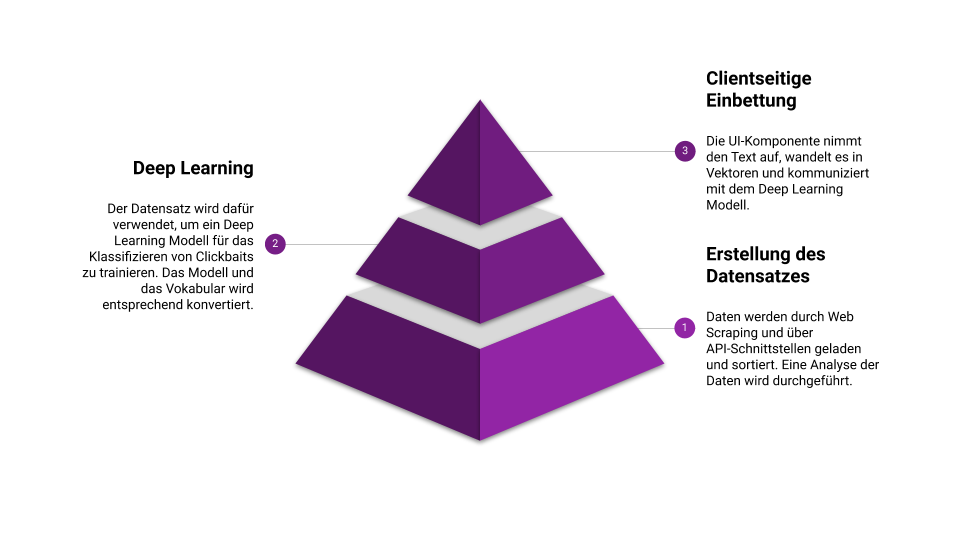
\includegraphics[width=15cm]{kapitel5/main_p.png}
    \caption[Darstellung der Konzeption]{Darstellung der Konzeption}
    \label{Kap5:Konzeption}
\end{figure}


Deep Learning Modelle benötigen eine große Menge an Beispielen um zu lernen. Es reicht außerdem nicht aus, nur eine große Menge an Daten zu beschaffen, sondern auch gute Daten auszuwählen. In der Studie von \cite*{Chakrabortya} haben die Autoren Daten aus dem Web geladen. Für die erste Kategorie, der Nicht-Clickbaits, wurde die Wikipedia-News-API verwendet. Um genug Beispiele für Clickbaits zu finden, sollten solche Medien herausgefunden werden. Um die Daten labeln zu können ist neben dem Titel eines Datenelementes auch die extraktion der Nachricht zu erfassen.

Die Wikipedia-News-API bietet einen Kostenlosen Endpunkt an, welches verschiedene Nachrichtenportale wie z.B. Politik, Wirtschaft, Kultur, Sport und Wissenschaft anbietet. Um Clickbaits zu finden verläuft die Datenaquise wesentlich schwieriger. Der Datensatz von \cite*{Chakrabortya} beinhalter jeweils 7500 Nachrichten je Kategorie. Es ist zu berücksichtigen, dass diese nicht mit Deep Learning Modellen arbeiten, sondern mit klassischen Machine Learning Algorithmen, die weniger Daten benötigen. Es müssen also mehr Daten her, also die Suche sollte neben den klassischen Clickbait-Seiten auch woanders erfolgen. Um die Datenextraktion zu automatisieren bietet sich die Software \enquote{Scrapy} an. Scrapy ist ein Open-Source Tool, welches das extrahieren von großen Mengen an Daten erleichtert. Es ist in Python geschrieben und kann durch seine Middleware Funktion auch die Daten direkt in eine SQL-Datenbank speichern.

Der mittlere Kern der Pyramide in Abbildung~\ref{Kap5:Konzeption} ist das Deep Learning Modell, welches als Inferenzmaschine betrachtet werden kann. Es wird durch Eingabe von gelabelten Daten trainiert und in ein entsprechendes Format gebracht. Es gibt mehrere Anbieter für das Deep Learning. Die meisten von Ihnen sind Open Source. Die bekanntesten Bibliotheken für das Deep Learning sind TensorFlow (welches von Google unterstützt wird) und PyTorch (welches von Facebook unterstützt wird). Seit März 2018 bietet TensorFlow die Möglichkeit, Modelle in der Programmiersprache JavaScript zu trainieren und zu benutzen. Ein klassischer Vorgang um Deep Learning Modelle dem Endbenutzer durch Webprogrammierung anzubieten war es immer, dass zunächst ein Modell trainiert wurde und dann auf einem Server geladen wurde. Der Server hatte dann einen Endpunkt, z.B. eine POST-Anfrage, welches eine Anfrage vom Clienten empfang. Diese Anfrage wurde dann im Server durch das Modell beantwortet und der Server sendete dem Clienten das Ergebnis. Durch TensorFlow.js ist es möglich erstens ein Modell komplett auf der Programmiersprache JavaScript zu entwickeln und zweitens es die Inferenzbildung durch einen Server in der Mitte nicht mehr nötig. Das Modell kann zusammen mit dem Framework in den Browser geladen werden und die bearbeitung erfolgt dort. In dieser Arbeit wurde das Modell nicht mit TensorFlow.js trainiert, da es auch möglich ist, Modelle in der konventionellen Weise mit der Keras API zu trainieren und dann in ein Webfreundliches Format umzuwandeln. Nach der Konversion können die Gewichte welches das Modell gerechnet hat und eine JSON-Datei, welches das Modell beschreibt hochgeladen und benutzt werden. Der Client muss nur noch diese Dateien in den Browser laden und kann dann selbst die Anfrage beantworten. Das trainieren auf konventionellen Wegen bietet außerdem den Vorteil, dass die Umgebung auf JavaScript nicht mit der Umgebung in Python konkurrieren kann. Die meisten Tools und Frameworks werden für Python geschrieben. Ein weiterer Grund ist, dass die bearbeitung auf dem heimischen Computer sehr langsam ist. Mit Google Colab können Deep Learning Modelle mit viel Rechnerkapazität trainiert werden.

Die Spitze der Pyramide macht die Benutzeroberfläsche aus. Diese wird komplett in JavaScript geschrieben. JavaScript ist die meistbenutze Programmiersprache und wird heute neben Webentwicklung auch auf dem Server verwendet. Mit TensorFlow.js ist es nun auch möglich, mit Tensors umzugehen. Die Schwierigkeit hier ist es, den Text, den der Benutzer eingibt, in Token und dann diese Token in Vektoren umzuwandeln, wenn das Modell keinen sogenannten \enquote{Input-Layer} hat welches einfache String einnehmen kann und diese umwandeln kann, dieses macht das Modell aber viel größer, da es eine größere Anzahl an Parametern hat und nicht Ziel dieser Arbeit. Eine andere Möglichkeit ist es, das gesamte Vokabular in einer JSON-Datei zu speichern und es der Benutzeroberfläsche zugänglich zu machen. Jedes auftauchende Wort im Vokabular bekommt einen Index, welches dann als \enquote{Übersetzer} dient und zur Umwandlung der Strings in Vektoren verwendet werden.




\section{Erstellung des Datensatzes}
\subsection{Erste Rohdatenbeschaffung durch Web Scraping}

Um einen Forschungsbeitrag zu leisten, hat diese Arbeit das Ziel ein Clickbait Corpus auf deutscher Sprache zu erstellen. Für die Erstellung eines solchen Korpus sind zunächst bestimmte Seiten einzugrenzen, die Clickbait Nachrichten anbieten. Die bekannteste Seite ist \enquote{buzzfeed} und \enquote{tasty}. Außerdem wurden auch Webseiten wie \enquote{web.de} oder \enquote{tv-movie}\footnote{Beinhaltet außerdem Schlagzeilen aus den Bereichen \enquote{tasty} und \enquote{quiz}} nach Clickbaits gescannt. Das Screening wurde am November 2020 durchgeführt. Um jedoch zu gewährleisten, dass die Nachrichten zeitlich weit außereinder liegen und somit eine größere Diversität haben, wurden Webseiten ausgewählt die Ihre Nachrichten in gewisser Weise Archivieren. Die gesammelten Daten reichen teilweise über ein Jahr zurück. Wie im Listing~\ref{Scrapy} unter in Zeile 12 zu sehen ist, besitzt die Seite im Beispiel eine Pagination-Funktion. Diese kann dafür verwendet werden, um auch ältere Nachrichten zu erfassen.

\begin{table}[h]
    \caption{Vergleich der Rohdaten nach dem Scrapingvorgang}
    \label{Datensatz_Herkunft}
    \renewcommand{\arraystretch}{1.2}
    \centering
    \sffamily
    \begin{footnotesize}
        \begin{tabular}{l l l}
            \toprule
            \textbf{Quelle}   & \textbf{Methodik} & Elemente \\
            \midrule
            de.wikinews.org   & API-Zugang        & 10.612   \\
            web.de            & Web Scraping      & 14.163   \\
            tvmovie.de        & Web Scraping      & 9.428    \\
            buzzfeed.de       & Web Scraping      & 798      \\
            promipool.de      & Web Scraping      & 26.779   \\
            heftig.de         & Web Scraping      & 605      \\
            frauenseite.net   & Web Scraping      & 148      \\
            bravo.de          & Web Scraping      & 7.476    \\
            \midrule
            Summe Clickbaits  &                   & 59.407   \\
            Summe Nachrichten &                   & 10.612   \\
            Summe insgesamt   &                   & 70.019   \\
            \bottomrule
        \end{tabular}
    \end{footnotesize}
    \rmfamily
\end{table}



Das Verfahren wurde automatisch mittels eines programmierten Scrapers je Seite durchgeführt. Ein Scraper ist ein Programm, welches Informationen aus einer Webseite automatisch extrahieren kann. Dieses gelingt, indem es nach HTML- oder CSS-Attributen oder sogar AJAX-Requests durchsucht oder diese imitiert. Im Listing~\ref{Scrapy} wird ein Web-Scraper vorgestellt. Scrapy führt in einer Schleife HTTP-Requests durch welche jeweils eine Antwort bekommen. Es können auch AJAX-Anfragen gesendet werden (z.B. ein POST-Request). Wenn die Anfrage Erfolgreich ist, kann die daraus resultierende Antwort auf bestimmte Eigenschaften und Attribute durchsucht werden (im Beispiel werden CSS-Attribute durchsucht). Diese Attribute beinhalten meisten die gewünschte Information, welches dann wie in der \texttt{parse\_url} und \texttt{parse\_page} Methode gezogen und in eine Datenbank gespeichert wird.



\begin{lstlisting}[language=Python,caption=Beispiel eines Scrapers]
import scrapy
from scrapy.http.request import Request
from datetime import datetime
from klickscraper.items import WebdeItem


class WebdeSpider(scrapy.Spider):
    name = "webde"
    scraped_at = datetime.now()

    def start_requests(self):
        for i in range(287):
            url = f"https://web.de/magazine/unterhaltung/stars/p{i}"
            yield Request(
                dont_filter=True,
                callback=self.parse_url,
                url=url)

    def parse_url(self, response):
        follow_ulrs = response.css(
            ".teaser-article__full").css("a::attr(href)").getall()
        for f in follow_ulrs:
            yield Request(
                url=f,
                dont_filter=True,
                callback=self.parse_page)

    def parse_page(self, response):
        if len(response.css("p::text").getall()) > 10:
            text = " ".join(response.css("p::text").getall())
        else:
            text = None
        yield WebdeItem(title=response.css('title::text').get(),
                        text=text,
                        scraped_at=self.scraped_at)
\end{lstlisting}\label{Scrapy}


\subsection{Explorative Datenanalyse der Rohdaten}
Um aus den Rohdaten Schlüsse über die sprachlichen Eigenschaften zu ziehen wird im folgenden Abschnitt eine explorative Datenanalyse durchgeführt. Um dies möglichst zu vereinfachen, wird der Rohdatensatz welches in einer SQL-Datenbank gespeichert wurde in ein Pandas\footnote{Pandas ist ein schnelles, flexibles und benutzerfreundliches Open-Source-Tool zur Analyse und Bearbeitung von Daten in Python.} Dataframe umgewandelt.
Aus der Abbildung~ist zu sehen, dass die Titel aus Wikinews länger sind. Neben der Länge der Schlagzeilen ist auch die Analyse der Wortauswahl wichtig. Aus der Literaturstudie können bestimmte Merkmale von Clickbaits festgestellt werden. Clickbaits enthalten meistens eine Frage oder Zahlen. Außerdem ist bei Clickbaits auch eine gewisse Wortauswahl festzustellen. Die Zuordnung der Wörter je Clickbait-Schlagzeile zu den Wortarten (Part-of-speech-Tagging oder POS-Tagging) wurde mittels der Python NLP-Bibliothek Spacy durchgeführt. Bei der Auswahl der Tags nachdem gesucht werden sollte, wurden die Erkenntnisse aus Kapitel 4 Berücksichtigt. Die Ergebnisse diese Analyse sind aus der Tabelle~\ref{pos} zu entnehmen.

\begin{table}[h]
    \caption{Vergleich der Ergebnisse des Part-of-speech-Taggings}
    \label{pos}
    \renewcommand{\arraystretch}{1.2}
    \centering
    \sffamily
    \begin{footnotesize}
        \begin{tabular}{l l l}
            \toprule
            \textbf{TAG}                  & \textbf{Auffälliges Wort (Häufigkeit)} \\
            \midrule
            ADJA  (attributives Adjektiv) & neu (1759), neue (1474)                \\
            ADJD   (adverbiales Adjektiv) & krass (171), wirklich  (349)           \\
            ADV   (Adverb)                & so (5142), endlich (357)               \\
            PDAT (Demonstrativpronomen)   & dies (3566)                            \\
            PROAV   (Pronominaladverb)    & darum (588), deshalb (251)             \\
            PWAT (Interrogativpronomen)   & welch (154)                            \\
            PWAV  (Relativpronomen)       & wie (488) warum (184)                  \\
            \bottomrule
        \end{tabular}
    \end{footnotesize}
    \rmfamily
\end{table}

% Eine eigene Analyse durch das Part-of-Speech_tagging mittels Scrapy ergibt einige Auffälligkeiten bezüglich der Clickbaits. Wörter wie \enquote{diese} (attribuierendes Demonstratives Pronomen), \enquote{warum} (adverbiales Interrogativ- oder Relativpronomen) oder \enquote{welche} (attribuierendes Interrogativpronomen) sind einige Auffällige Tags aus den Schlagzeilen der Clickbaits.



% \begin{lstlisting}[language=Python,caption=Funktion zur Umwandung der Datenbank in en Pandas Dataframe]
% def connect_to_db(tablename, db_path):
%     return pd.read_sql_query(
%         f"SELECT * FROM {tablename}", sqlite3.connect(db_path))
% \end{lstlisting}\label{Pandasdb}


\begin{figure}[H]
    \centering
    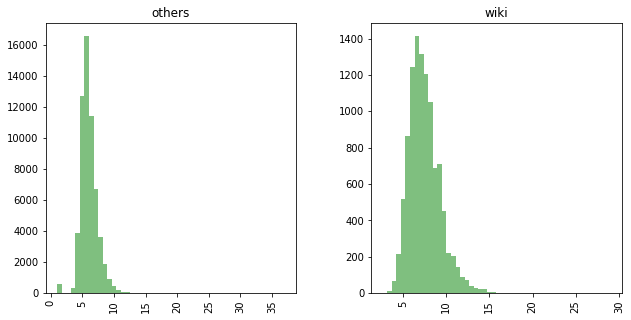
\includegraphics[width=14cm]{kapitel5/hist2.png}
    \caption[Vergleich der Wortlängen der Rohdaten]{Vergleich der Wortlängen, das Histogramm rechts (Wikinews) ist breiter als das Histogramm links (Clickbaits)}
    \label{Kap5:Hist2}
\end{figure}

% \begin{figure}[H]
%     \centering
%     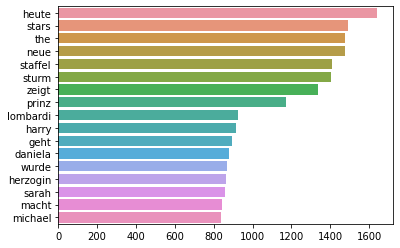
\includegraphics[width=10cm]{kapitel5/freq_word1.png}
%     \caption[Häufigsten Wörter aus den Rohdaten der Clickbaits Titel]{Die Darstellung zeigt das Aufkommen der Häufigsten Wörter aus den Titeln der Clickbaits}
%     \label{Kap5:freq1}
% \end{figure}

% \begin{figure}[H]
%     \centering
%     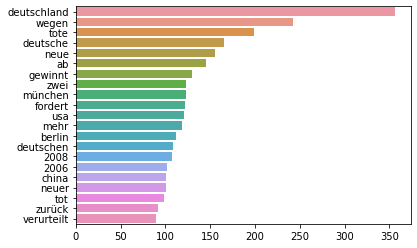
\includegraphics[width=10cm]{kapitel5/freq_word2.png}
%     \caption[Häufigsten Wörter aus den Rohdaten der Wikinews Titel]{Die Darstellung zeigt das Aufkommen der Häufigsten Wörter aus den Titeln der Wikinews Nachrichten}
%     \label{Kap5:freq2}
% \end{figure}


\subsection{Labeln der Daten}
Aus der Tabelle~\ref{Datensatz_Herkunft} ist zu entnehmen, dass ca. 60.000 potenzielle Clickbaits vorhanden sind. Um dieses nicht per Hand labeln zu müssen besteht der Ansatz darin, bestimmte Muster zu erkennen und diese Muster auszunutzen, um die Anzahl der Kandidaten auf ein entsprechendes niedriges Niveau zu bringen. Die Literaturstudie und die explorative Datenanalyse bringen gemeinsam folgende Schlüsse:

\begin{enumerate}
    \item Clickbaits sind meisten Fragen wie \enquote{Welcher Schuh passt dir am meisten?}
    \item Clickbaits enthalten meistens Zahlen in Form eines Listings \enquote{Das sind die 10 schnellsten Autos}
    \item Clickbaits haben eine niedrigere Wortlänge als normale Nachrichten
    \item Clickbaits beinhalten einige für sie markanten Wörter wie \enquote{diese} oder \enquote{so}
\end{enumerate}

Diese Erkenntnisse können programmatisch umgewandelt werden und somit der Rohdatensatz um ein vielfaches reduziert werden.


\begin{lstlisting}[language=Python,caption=Funktion welches ein Dataframe je nach Argumenten labelt]
def contains_word(word, row):
    for r in row:
        if r in word:
            return 1


def label_data_with_arg(df, col_name, arg_):
    return df[col_name].apply(
        lambda x: contains_word(arg_, re.findall(r"[\w']+|[.,!?;]", x.lower())))
\end{lstlisting}\label{Label1}

\begin{lstlisting}[language=Python,caption=Funktionen für durchschnittliche Wortlänge und Interpunktion]
import re
import string


def remove_punc(text):
    text = re.sub('\[.*?\]', '', text)
    text = re.sub('https?://\S+|www\.\S+', '', text)
    text = re.sub('<.*?>+', '', text)
    text = re.sub('[%s]' % re.escape(string.punctuation), '', text)
    text = re.sub('\n', '', text)
    text = re.sub('\w*\d\w*', '', text)
    return text

def get_avg_length(string):
    words = remove_punc(string).split()
    try:
        count = int(sum(len(word) for word in words) / len(words))
    except ZeroDivisionError:
        count = 1
    return count
\end{lstlisting}\label{Label2}

\begin{lstlisting}[language=Python,caption=Tagger Funktion]
import spacy
nlp = spacy.load('de')


def contains_pos(sentence):
    list_ = ["PDAT", "ADJD", "ADJA", "PIS", "PWAV", 
            "PTKA", "VAFIN", "PROAV", "ADV"]
    doc = nlp(sentence)
    for token in doc:
        if str(token.tag_) in list_:
            return "1"

def label_data_with_pos(df, col_name):
    return df[col_name].apply(
        lambda x: contains_pos(x.lower()))
\end{lstlisting}\label{Label3}


\subsection{Analyse der Daten}
Die Summe der Wikinews Nachrichten beträgt ca. 10.000. Mit der Zugabe weiterer 10.000 Clickbaits, die durch das labeln entstehen, ergibt sich ein Datensatz mit 20.000 Beispielen. Die Tabelle~\ref{data} verschafft einen Übrerblick über alle Daten. Interessant ist bei den Clickbaits, dass ca. 33\% aller Clickbaits ein Fragezeichen oder eine Zahl beinhalten und ca. die hälfte aller Daten im Datensatz ein bestimmtes Tag wie \enquote{diese} oder \enquote{so} enthalten. Bei den Wikinews Nachrichten liegen diese Anteile deutlich unten. Alle drei genannten Eigenschaften liegen unter 1\%. Die durchscnittliche Wortlänge beträgt bei den Clickbaits bei 5, während bei den Wikipedia Nachrichten dieses bei 7 liegt.

\begin{table}[h]
    \caption{Beschreibung des gelabelten Datensatzes}
    \label{data}
    \renewcommand{\arraystretch}{1.2}
    \centering
    \sffamily
    \begin{footnotesize}
        \begin{tabular}{l l l l l l}
            \toprule
                           & \textbf{has\_question} & \textbf{has\_keyword} & \textbf{has\_number} & \textbf{avg\_word\_length} & \textbf{label} \\
            \textbf{count} & 20000                  & 20000                 & 20000                & 20000                      & 20000          \\
            \textbf{mean}  & 0.1782                 & 0.3190                & 0.0854               & 6.1307                     & 0.5000         \\
            \textbf{std}   & 0.3826                 & 0.4661                & 0.2795               & 1.7874                     & 0.5000         \\
            \textbf{min}   & 0                      & 0                     & 0                    & 1.0000                     & 0              \\
            \textbf{max}   & 1                      & 1                     & 1                    & 27.0000                    & 1              \\

            \bottomrule
        \end{tabular}
    \end{footnotesize}
    \rmfamily
\end{table}

Bei der Betrachtung der Wörter mit der Word-Cloud Analyse können bestimmte Themen, die die Titel zürückgeben betrachtet werden.  Auffällig sind neben Promis auch die Wörter \enquote{darum}, \enquote{quiz} \enquote{sieht} und \enquote{macht}. Bei den Wikipedia Nachrichten geht es mehr um Deutschland und der Welt.


\begin{figure}[H]
    \centering
    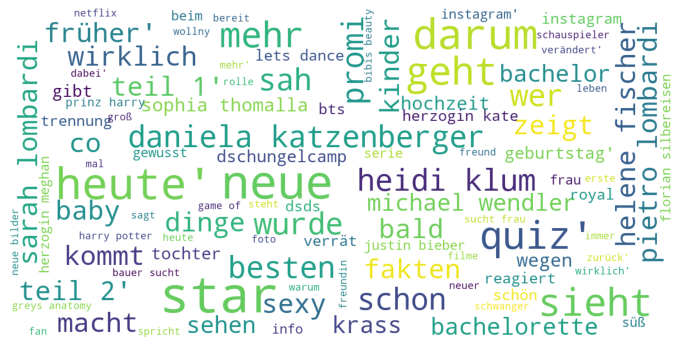
\includegraphics[width=12cm]{kapitel5/wo_click.png}
    \caption[Word Cloud Analyse für die Clickbaits Schlagzeilen]{Die Darstellung zeigt das Aufkommen der Häufigsten Wörter aus den Titeln der Wikinews Nachrichten}
    \label{Kap5:clwc}
\end{figure}

\begin{figure}[H]
    \centering
    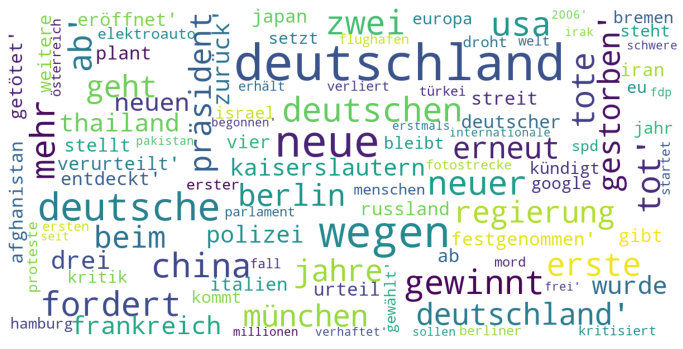
\includegraphics[width=12cm]{kapitel5/news.png}
    \caption[Word Cloud Analyse für die Wikinews Schlagzeilen]{Die Darstellung zeigt das Aufkommen der Häufigsten Wörter aus den Titeln der Wikinews Nachrichten}
    \label{Kap5:clwc}
\end{figure}


\section{Das Deep Learning Modell}
\subsection{Einleitung}
\subsection{Soft- und Hardware}
\textit{TensorFlow} ist eine Bibliothek, mit der Deep Learning durchgeführt werden können, es wurde im Jahr 2015 von Google Open Source gemacht. Mit TensorFlow werden die Datan als Tensoren dargestellt und fließen durch Schichten. Dieses ermöglicht die Inferent und das Traiing in maschinellen Lernmodellen. Ein Tensor ist ein multidimensionales Array. In neuronalen Netzen und beim Deep Learning wird jedes Datenelement und jedes Berechnungsergebnis als Tensor dargestellt, z.B. kann ein Graustufenbild als 2-Dimensionales-Array dargstellt werden oder ein Farbbild als 3-Dimensionales-Array. Der Tensor kann unterschiedliche Datentypen haben (z. B. float32 oder int32). Neben dem Typen eines Tensors gibt es die zweite Eigenschaft, die Form eines Tensors. Die Form eines Tensors gibt die Größe des Tensors entlang aller seiner Abmessungen an. Beispiel: Ein 2-Dimensionales-Tensor hat die Form (128, 256). Ein Tensor kann unabhängig von den ursprünglichen Daten in ein sogenanntes Layer eingespeist werden, welches nur danach schaut, welcher Datentyp und Form der Tensor hat. Tensoren sind also eine Art Container die Daten organisieren und dafür verwendet werden können, dass diese parallel verarbeitet werden können.


\begin{lstlisting}[language=Python,caption=Beispiel eines Tensors in TensorFlow]
import tensorflow as tf


rank_2_tensor = tf.constant([[1, 2],
                             [3, 4],
                             [5, 6]], dtype=tf.float16)
\end{lstlisting}\label{Label3}

Um den zweiten Ausdruck in \enquote{TensorFlow} zu verstehen muss der Tensor als eine Art \enquote{Flüssigkeit} vorgestellt werden, welches die Daten trägt. In TensorFlow fließt es durch ein Diagramm - eine Datenstruktur, die aus miteinander verbundenen mathematischen Operationen (Knoten genannt) besteht. Wie Abbildung~\ref{tnflayers} zeigt, kann der Knoten aufeinanderfolgende Schichten in einem neuronalen Netzwerk sein. Jeder Knoten nimmt Tensoren als Eingaben und erzeugt Tensoren als Ausgaben. Die \enquote{Flüssigkeit} wird in verschiedene Formen und Werte umgewandelt, wenn sie durch das TensorFlow-Diagramm \enquote{fließt}. Dies entspricht der Transformation von, d.h. dem Kern dessen, was neuronale Netze tun. Mit TensorFlow können Ingenieure für maschinelles Lernen alle Arten von neuronalen Netzen schreiben, von flachen bis zu sehr tiefen, von CNN für Computer Vision bis zu wiederkehrenden neuronalen Netzen (RNNs) für Sequenzaufgaben .

 \begin{figure}[H]
     \centering
     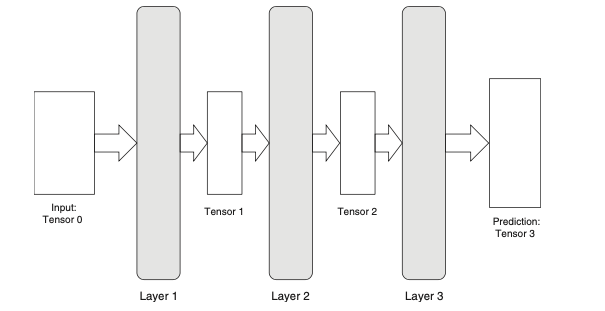
\includegraphics[width=10cm]{kapitel5/tflayers.png}
     \caption[Die Darstellung eines Deep Learning Modells in Tensorflow]{Die Darstellung eines Deep Learning Modells in Tensorflow - Die Tensoren fließen durch jede Schciht im Modell durch (Abbildung aus)}
     \label{Kap5:tnflayers}
 \end{figure}


Im Kern wurde TensorFlow sehr allgemein und flexibel konzipiert: Die Operationen können beliebige genau definierte mathematische Funktionen sein, nicht nur Schichten neuronaler Netze. Dies können beispielsweise mathematische Operationen auf niedriger Ebene sein, beispielsweise das Addieren und Multiplizieren von zwei Tensoren - die Art von Operationen, die innerhalb einer neuronalen Netzwerkschicht stattfinden. Dies gibt Deep-Learning-Ingenieuren und -Forschern die Möglichkeit, beliebige und neuartige Operationen für Deep-Learning zu definieren. Für einen großen Teil der Deep-Learning-Praktiker ist die Manipulation solcher Maschinen auf niedriger Ebene jedoch schwieriger als es sich lohnt. Dies führt zu aufgeblähtem und fehleranfälligerem Code und längeren Entwicklungszyklen. Die meisten Deep-Learning-Ingenieure verwenden eine Handvoll fester Schichttypen (z. B. Faltung, Pooling oder Dichte). In seltenen Fällen müssen neue Ebenentypen erstellt werden. Hier ist die LEGO-Analogie angebracht. Bei LEGOs gibt es nur wenige Blocktypen. LEGO Builder müssen nicht darüber nachdenken, was nötig ist, um einen LEGO Block zu erstellen. Dies unterscheidet sich von einem Spielzeug wie beispielsweise Play-Doh, das der Low-Level-API von TensorFlow entspricht.

Die Fähigkeit, LEGO-Blöcke zu verbinden, führt jedoch zu einer kombinatorisch großen Anzahl von Möglichkeiten und einer praktisch unendlichen Leistung. Es ist möglich, ein Spielzeughaus mit LEGOs oder Play-Doh zu bauen. Wenn Sie jedoch keine besonderen Anforderungen an Größe, Form, Textur oder Material des Hauses haben, ist es viel einfacher und schneller, es mit LEGOs zu bauen. Für die meisten von uns wird das LEGO-Haus, das wir bauen, stabiler stehen und schöner aussehen als das Play-Doh-Haus, das wir bauen würden.

In der Welt von TensorFlow ist das LEGO-Äquivalent die High-Level-API namens Keras.  Keras bietet eine Reihe der am häufigsten verwendeten Arten von neuronalen Netzwerkschichten mit jeweils konfigurierbaren Parametern. Außerdem können Benutzer die Schichten miteinander verbinden, um neuronale Netze zu bilden. Darüber hinaus enthält Keras auch APIs für

\begin{itemize}
     \item Festlegen, wie das neuronale Netzwerk trainiert werden soll (Verlustfunktionen, Metriken und Optimierer)
     \item Daten einspeisen, um das neuronale Netzwerk zu trainieren oder auszuwerten oder das Modell zur Inferenz zu verwenden
     \item Überwachung des laufenden Schulungsprozesses (Rückrufe)
     \item Modelle speichern und laden
     \item Drucken oder Plotten der Architektur von Modellen
 \end{itemize}



Mit Keras können Benutzer den gesamten Deep-Learning-Workflow mit sehr wenigen Codezeilen ausführen. Mit der Flexibilität der Low-Level-API und der Verwendbarkeit der High-Level-API bilden TensorFlow und Keras ein Ökosystem, das im Bereich der Deep-Learning-Rahmenbedingungen hinsichtlich der industriellen und akademischen Akzeptanz führend ist. Als Teil der anhaltenden Deep-Learning-Revolution sollte ihre Rolle, Deep Learning einem breiteren Publikum zugänglich zu machen, nicht unterschätzt werden. Vor Frameworks wie TensorFlow und Keras konnten nur diejenigen mit CUDA-Programmierkenntnissen und umfassender Erfahrung im Schreiben neuronaler Netze in C++ praktisches Deep Learning durchführen. Mit TensorFlow und Keras ist es viel weniger erforderlich, GPU-beschleunigte tiefe neuronale Netze zu erstellen.

Es gab jedoch ein Problem: Es war nicht möglich, TensorFlow- oder Keras-Modelle in JavaScript oder direkt im Webbrowser auszuführen. Um Deep-Learning-Modelle im Browser bereitzustellen, musste dies über HTTP-Requests an einen Backend-Server getan werden. TensorFlow.js löst dieses Problem. Die JavaScript-API hat eine Keras-ähnliche High-Level-API welches auf dem Low-Level-Kern erstellt wurde, die es Benutzern erheblich erleichtert, Deep-Learning-Modelle in der JavaScript-Bibliothek zu definieren, zu trainieren und auszuführen. Um die Interoperabilität weiter zu verbessern, wurden Konverter erstellt, mit denen TensorFlow.js aus TensorFlow und Keras gespeicherte Modelle importieren und Modelle in diese exportieren kann.


\textit{Google Colab} ist ein kostenloser Cloud-Dienst auf Basis von Jupyter Notebooks, der GPU unterstützt. Dies ist nicht nur ein  Tool zur Verbesserung der Codierungsfähigkeiten, sondern ermöglicht es auch absolut jedem, Deep-Learning-Anwendungen mit gängigen Bibliotheken wie PyTorch, TensorFlow, Keras und OpenCV zu entwickeln.

 \begin{figure}[H]
     \centering
     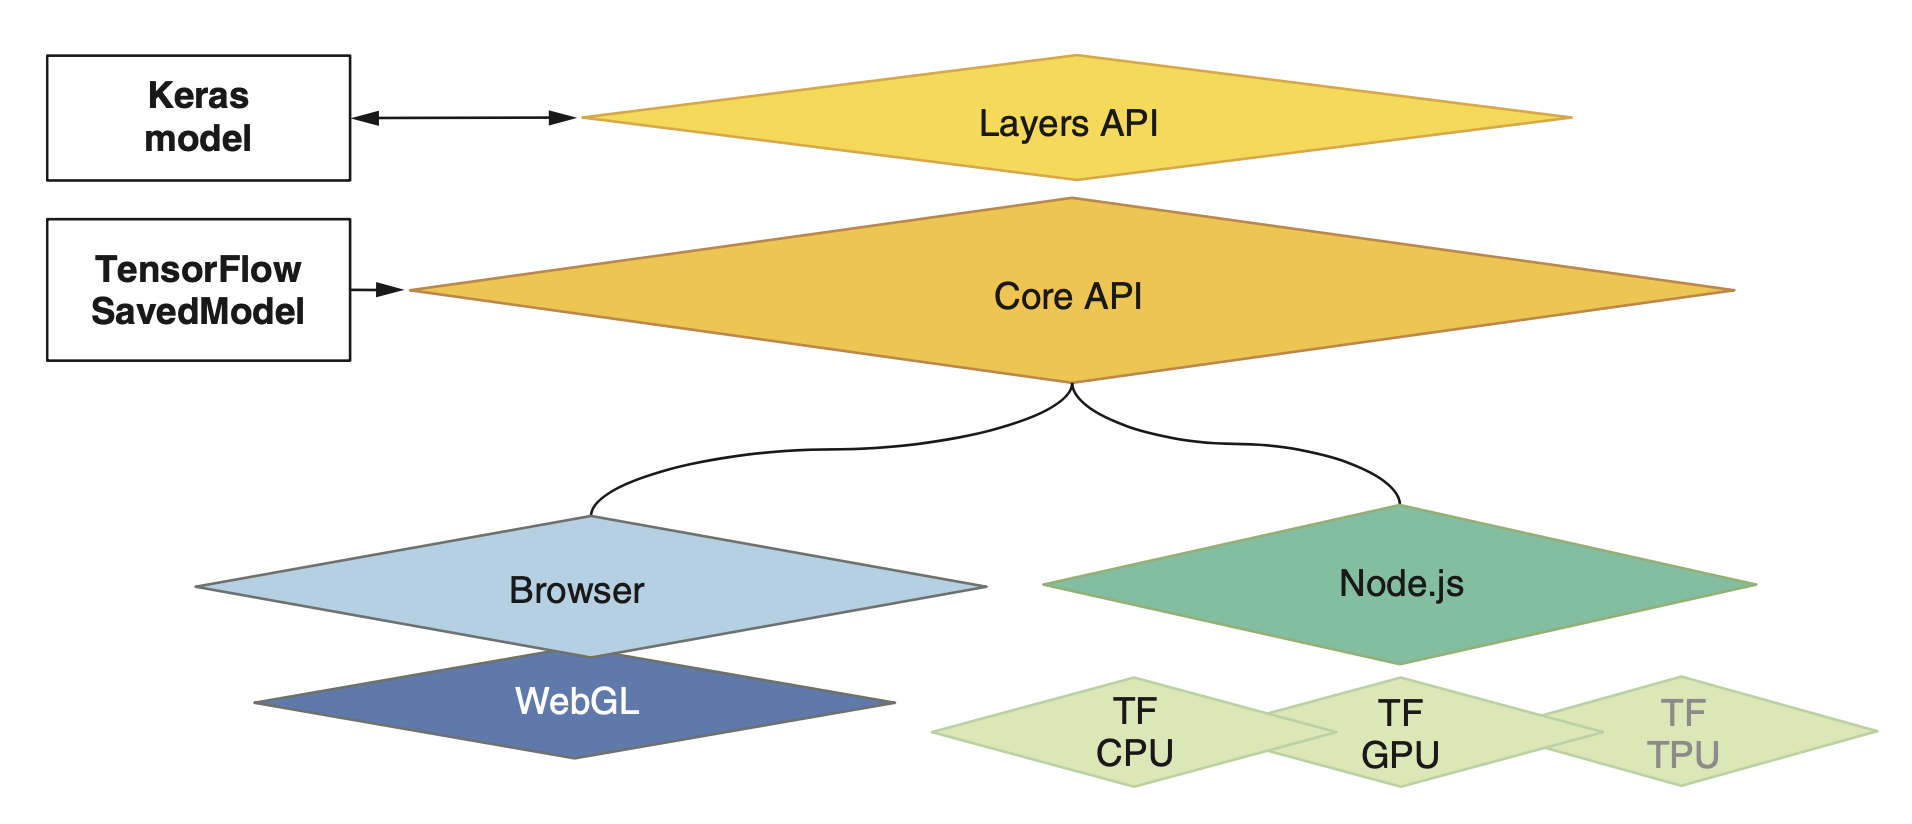
\includegraphics[width=12cm]{kapitel5/tfjsarch.png}
     \caption[Die Architektur von TensorFlow.js]{Die Architektur von TensorFlow.js - Abbildung zeigt die Verhältnisse zwischen der Paython API von TensorFlow und Keras mit TensorFlow.js}
     \label{Kap5:tfjsarch}
 \end{figure}

\subsection{Preporcessing}
Beim Preprocessing der Daten sollte der Text umgewandelt werden, sodass ein Training erfolgen kann. Bei der Erstellung des Datensatzes wurden die Titel weitestgehend gesäubert. Bei einigen Schlagzeilen waren neben dem Titel auch Namen der Seite vorhanden, diese wurden entfernt. Jedoch sollte der Text, wenn noch nicht erfolgt, in Kleinbuchstaben umgewandelt werden. Die Leerzeichen nach und vor dem jeweiligen Satzzeichen sollte getrennt werden. Da bei Clickbaits Satzzeichen wie Fragezeichen oder Ausrufezeichen eine Beudeutung hat werden diese nicht vollständig entfernt und in den Vokabular aufgenommen. Stoppwörter sind bieten normalerweise keine große Relevanz, sind hier jedoch bedeutsam, z.B. Präpositionen.

Beim Preprocessing wird auch der Datensatz in zwei Hälften, des Trainingssatz und des Testsatz aufgeteilt. Es ist üblich dieses in einer Ratio von 0.8/0.2 auszuführen. Das Ziel ist es vorherzusagen, ob eine bestimmte Schlagzeile Clickbait ist oder nicht. Dieses Bedeutet, dass nach der Entwicklung des Modells Vorhersagen über neue Textüberprüfungen getroffen werden muss. Dieses erfordert, dass für diese neue Überprüfung dieselbe Datenvorbereitung durchgeführt wird, wie für die Trainingsdaten für das Modell. Um sicherzustellen, dass diese Einschränkungen in die Bewertung der Modelle integriert wird, wird vor jeder Datenaufbereitung der Datensatz, in Trainings- und Testsatz aufgeteilt. In der Funktion~\ref{TrainTestFunc} wird der Datensatz aus einer CSV-Datei gelesen und mittels Pandas in ein Dataframe umgewandelt. Es werden zufällig 80\% der Titel \enquote{maskiert} und entsprechend aufgeteilt und als Tupel zurückgegeben. Es entstehen somit ca. 16.000 Beispiele für das Training und 4.000 Beispiele für das Testen.

\begin{lstlisting}[language=Python,caption=Funktion für das Aufteilen des Datensatzes]
import pandas as pd
import numpy as np


def create_train_test(csv_file_path):
    dataframe_ = pd.read_csv(csv_file_path).drop_duplicates()
    msk = np.random.rand(len(dataframe_)) < 0.8
    train = dataframe_[msk]
    test = dataframe_[~msk]
    test.reset_index(drop=True)
    train.reset_index(drop=True)
    return train, test;
\end{lstlisting}\label{TrainTestFunc}

Im Listing~\ref{CleanFunct} werden die Buchstaben in klein gesetzt und alles was nicht gewünscht wird entfernt. Um die Fragezeichen und Ausrufezeichen wird ein Leerzeichen gesetzt, damit diese vom jeweilligen Wort getrennt werden können. Auf das Entfernen der Stoppwörter wird verzichtet, da diese wichtige Informationen über Clickbaits Schlagzeilen geben können.

\begin{lstlisting}[language=Python,caption=Die Preprocessing-Funktion]
import re


def text_cleaner(text):
    newtext = re.sub(r'[^A-Za-z?!.0-9üäöß]+', ' ', text)
    newtext = re.sub('([!?])', r' \1 ', newtext)
    newtext = re.sub('\s{2,}', ' ', newtext)
    return newtext.lower()
    
    
train["Title"] = train["Title"].apply(lambda x: text_cleaner(x))
test["Title"] = test["Title"].apply(lambda x: text_cleaner(x))
\end{lstlisting}\label{CleanFunct}

\subsection{Das Erstellen Einbetten eines Vokabulars}


Es ist wichtig ein Vokabular bekannter Wörter zu definieren, wenn One-Hot-Encoding oder ein Einbettungsmodell verwendet wird. Je mehr Wörter vorhanden sind, desto größer ist die Darstellung von Dokumenten. Daher ist es wichtig, die Wörter nur auf diejenigen zu beschränken, von denen angenommen wird, dass sie vorhersagbar sind. Dies ist im Voraus schwer zu wissen und oft ist es wichtig, verschiedene Hypothesen zum Aufbau eines nützlichen Vokabulars zu testen. Aus dem vorherigen Abschnitt wurde einige Interpunktion (alles außer Fragenzeichen und Ausrufezeichen und Punkt) entfernt. Zahlen wurden nicht entfernt und auch Stoppwörter sind dem Datensatz enthalten. Es kann also aus allen Schlagzeilen eine Reihe aller bekannten Wörter ermittelt werden. Jedes Element im Vokabular wird als Zahl dargestellt. Es handelt sich also um eine Wörterbuchzuordnung von Wörtern und deren Index. Somit kann das Wort auf eine einfache Weise aktualisiert und abgefragt werden.

Keras bietet eine Klasse namens \texttt{Tokeniser} welches diesem Zwecke dient. Diese Klasse ermöglicht die Vektorisierung eines Textkorpus, indem jeder Text entweder in eine Folge von Ganzzahlen (jede Ganzzahl ist der Index eines Tokens in einem Wörterbuch) oder in einen Vektor umgewandelt wird, in dem der Koeffizient für jedes Token basierend auf der Wortanzahl binär sein kann. Der Tokeniser basiert auf der tf-idf Methode.

Die Methode \texttt{fit\_on\_texts} dieser Klasse wird aktualisiert den internen Wortschatz anhand einer Liste von Texten. Um den Text in eine Folge von ganzen Zahlen umzuwandeln ist das Ausführen der Methode \texttt{fit\_on\_texts} zwingend erforderlich. Dann kann mit der Methode \texttt{texts\_to\_sequences} die häufigsten auftretenden Wörter die dem Tokeniser bekannt sind berücksichtigt.

Der nächste Schitt ist das Padding. Mit der Methode \texttt{pad\_sequences} kann eine Liste von Sequenzen mit einer bestimmten Länge in ein 2-Dimensionales-Numpy-Array umgewandelt werden. Sequenzen die länger als die angegebene maximale Länge sind werden abgeschnitten, damit sie der gewünschten Länge entsprechen. Sequenzen die kürzer sind wiederum, werden mit einer Null aufgefüllt, bis sie dem maximalen Wert entsprechen. Das Vorabfüllen oder Entfernen von Werten am Anfang der Sequenz ist die Standardeinstellung. Es wird festgestellt, dass die Titel im Datensatz eine maximale Tokenlänge von 21 haben. Die maximale Länge wird auf 40 Tokens gesetzt. Es wird also nachher erlaubt, eine Abfrage mit maximal 40 Wörtern oder Tokens durchzuführen. Der Tokeniser gibt somit z.B. für den Titel \enquote{die 10 besten apps für mädchen} einen Array der Länge 30, wobei die ersten 24 Werte eine Null enthalten und die restlichen 6 eine bestimmte Zahl, welches den Index des im String enthaltenen Wörtes darstellt. 



\begin{lstlisting}[language=Python,caption=Die Tokeniser-Funktion]
from keras.preprocessing.text import Tokenizer
from keras.preprocessing.sequence import pad_sequences


def tokenize_text(train_df, test_df, max_l):
    tokenizer = Tokenizer()
    tokenizer.fit_on_texts(train_df)
    vocab_size = len(tokenizer.word_index) + 1
    tokenized_text_train = pad_sequences(
        tokenizer.texts_to_sequences(train_df), maxlen=max_l)
    tokenized_text_test = pad_sequences(
        tokenizer.texts_to_sequences(test_df), maxlen=max_l)
    return {"tokenized_text_train": tokenized_text_train, "tokenized_text_test": tokenized_text_test, "vocab_size": vocab_size, "tokenizer": tokenizer}
\end{lstlisting}\label{TokenizerFunc}

%Es basiert auf TFIDF ==> aufmahme in den teoretischen Teil
% curse of dimeniolaty in teoretischen teil nehmen
% FOrmel sind nicht on flow mit den zahlen

Eine Worteinbettung ist eine Möglichkeit, Text darzustellen, bei der jedes Wort im Vokabular durch einen reellen Vektor in einem hochdimensionalen Raum dargestellt wird. Die Vektoren werden so gelernt, dass Wörter mit ähnlichen Bedeutungen eine ähnliche Darstellung im Vektorraum haben (nahe im Vektorraum). Dies ist eine aussagekräftigere Darstellung für Text als klassische, bei denen Beziehungen zwischen Wörtern oder Token ignoriert oder in Bigram- und Trigramm-Ansätzen erzwungen werden. Die Vektordarstellung für Wörter kann während des Trainings des neuronalen Netzwerks gelernt werden. Dieses kann in der Keras Deep Learning-Bibliothek mithilfe der Einbettungsebene ausgeführt werden. 


Die Keras-Einbettungsschicht erfordert Ganzzahl-Eingaben, bei denen jede Ganzzahl einem einzelnen Token zugeordnet ist, das eine bestimmte reelle Vektordarstellung innerhalb der Einbettung aufweist. Diese Vektoren sind zu Beginn des Trainings zufällig, werden jedoch während des Trainings für das Netzwerk von Bedeutung. Durch die Funktionen aus Listing~\ref{CleanFunct} und Listing~\ref{TokenizerFunc} wurde das Encoding ausgeführt. Schließlich werden die Klassenbezeichnungen für den Trainingsdatensatz und Testdatensatz definieren, die für das überwachte neuronale Netzwerkmodell erforderlich sind, um die Clickbaits vorherzusagen. Die Daten werden zuletzt in ein TensorFlow dataset umgewandelt, um sie leichter in Keras einzuspeisen. Somit entsteht ein Datensatz zum training mit einem gesamten Vokabular von ca. 23.000 Vokabeln und einer erwarteten maximalen Eingangslänge von 30 Wörtern.

Die Daten wurden in den frühereren Etappen in \enquote{Train} und \enquote{Test} aufgeteilt. Mit der Funktion aus Listing~\ref{LabelFunc} werden die Labels \textit{Clickbait 0} und  \textit{News 1} in ein Array umgewandelt, um sie später in mittels \texttt{tensorflow\_datasets} umzuwandeln, gemeinsam mit den Arrays der Tokens (siehe Listing~\ref{DataSet)}. Der Grund für diese Konversion ist, dass diese Daten viel einfacher codiert und encodiert werden können, als z.B. mit Pandas Dataframes (siehe Listing~\ref{TrainModel}).


\begin{lstlisting}[language=Python,caption=Die Label-Funktion]
def create_labels(train_data, test_data):
    encoded_labels = preprocessing.LabelEncoder()
    y = encoded_labels.fit_transform(train_data['label'])
    y = to_categorical(y)
    y_test = encoded_labels.transform(test['label'])
    y_test = to_categorical(y_test)
    return y, y_test;

y, y_test = create_labels(train, test)
\end{lstlisting}\label{LabelFunc}

\begin{lstlisting}[language=Python,caption=Die Dataset Erstellung]
import tensorflow_datasets as tfds

train_dataset = tf.data.Dataset.from_tensor_slices((tokenized_text_train, y))
test_dataset = tf.data.Dataset.from_tensor_slices((tokenized_text_test, y_test))
\end{lstlisting}\label{DataSet}





\subsection{Das Erstellen eines Modells}



In Listing~\ref{BuildModel} wird ein sequentielles Modell erstellt. Diesem Modell kann durch die Methode \texttt{add} jeweils eine Schicht angehängt werden, und Keras arbeitet dieses nacheinander ab. Die API von Keras von Keras wird verwendet um das Modell zusammen zu bauen. Die Definitionen der einzelnen Methoden mit der das Modell gebaut und trainiert wurde, sind aus der Dokumentation von Google\citep{google1} entnommen. Dort werden viele Begriffe, die im Zusammenhang mit dem bauen und trainieren eines Deep Learning oder Machine Learning Modells stehen erklärt. Aus diesem Grund wird in diesem und nächsten Abschnitt auf diese Quelle verwiesen.

Zunächst mussen aber einige Parameter festgelegt werden. Diese sind \texttt{loss} also die Verlustfunktion, \texttt{metric} also nach welchen Metriken das Modell bemessen werden soll und \texttt{opt} der \texttt{Optimizer} wodurch das Modell lernt. Da es sich um eine binäre Klassifikation handelt wurden diese entsprechend den Parameteren ergänzt. Da es eine binäre Klassifikation ist, wird wird die \texttt{BinaryCrossentropy} verwendet. Als Optimizer wurde \texttt{Adam} ausgewählt. Die Lernrate ist ein Skalar, mit dem ein Modell über einen Gradientenabstieg trainiert wird. Während jeder Iteration multipliziert der Gradientenabstiegsalgorithmus die Lernrate mit dem Gradienten. Das resultierende Produkt wird als Gradientenschritt bezeichnet. Die Lernrate ist ein wichtiger Hyperparameter. Ein Optimizer ist eine spezifische Implementierung des Gradientenabstiegsalgorithmus. Die Basisklasse von TensorFlow für Optimierer ist tf.train.Optimizer. Beliebte Optimierer sind \texttt{AdaGrad}, das für ADAptive GRADient Abstammung steht und \texttt{Adam}, der für ADAptive with Momentum steht. Hyperparameter können dafür verwendet werden, um das Modell zu justieren und es gibt keine wirklichen Regel bei dem Konsum dieser Paramater. 

Nachdem die Hyperparameter popularisiert wurden, wird dem Modell die erste Schicht zugeführt. Dieses ist die Einbettungsschicht. Die Worteinbettung sind eine Möglichkeit, ein Wort als Vektor darzustellen (ein 1D-Tensor in TensorFlow). Durch Worteinbettungen können jedoch die Werte der Elemente des Vektors trainiert werden, anstatt nach einer Regel wie der Wort-zu-Index-Zuordnung in One-Hot-Codierung fest codiert zu werden. Mit anderen Worten, wenn ein textorientiertes neuronales Netzwerk die Worteinbettung verwendet, werden die Einbettungsvektoren zu trainierbaren Gewichtungsparametern des Modells. Sie werden durch dieselbe Backpropagation-Regel wie alle anderen Gewichtungsparameter des Modells aktualisiert. Es gibt auch die Möglichekeit, eine vortrainierte Einbettungsschicht zu nehmen. Diese werden auf viel größere Mengen an Daten trainiert und können für vielseitige Zwecke verwendet werden, ohne dass von Grunde aus neu trainiert werden muss. In diese Fall trainiert das Modell die Einbettungen selbst, anstatt sich auf die vorab trainierten Einbettungen zu verlassen.


Um das Modell vor dem Overfitting zu schützen gibt es bestimmte Strategien, die angewendet werden können. Dieses sind sogenannte Regularisierungstrategien. Es kann als eine Art \enquote{Strafe} betrachtet werden, für die Komplexität des Modells. Da bei wenig Daten und hoher Komplexität das Modell nicht wirklich lernt, sondern sich den gegebenen wenigen Daten \enquote{überanpasst} können diese dagegen wirken. Die L2-Regularisierung ist eine Art der Regularisierung, die Gewichte proportional zu Summe der Quadrate der Gewichte bestraft. Die L2-Regulariserung hilft dabei, Ausreißergwichte (mit hohen positiven oder niedrigen negativen Weten) näher an 0, aber nicht ganz an 0 zu bringen (im gegensatz zur L1-Regularisierung). Die L2-Regularisierung verbessert immer die Generalisierung in linearen Modellen. Die L1-Regularisierung bestaft die Gewichte proportional zur Summe der absoluten Werte der Gewichte. In Modellen, die auf spärlichen Merkmalen basieren, hilft die L1-Regularisierung dabei, die Gewichtung irrelevanter oder kaum relevanter Merkmale auf genau 0 zu bringen, wodurch diese Merkmale aus dem Modell entfernt werden.

Die \texttt{Conv1D}-Ebene wird verwendet um die Faltung durchzuführen. Eine CNN ist ein neuronales Netzwerk, in dem mindestens eine Schicht die Faltungsschicht ist. Ein typisches neuronales Faltungsnetzwerk besteht aus einer Kombination der von Faltungsschichten, Poolingschichten, und vollständig verbundene Schichten. Die Faltungsschicht hier ist eine eindimensionale Faltungsschicht. Bestimmte Muster aus dem Text werden hier erkannt (z.B. ob nach einem negativen Verb ein bestimmtes Wort auftaucht. In dem Beispiel gibt es 32 Filter. Beim maschinellen Lernen werden Faltungsfilter normalerweise mit Zufallszahlen gesetzt, und dann trainiert das Netzwerk die idealen Werte. Die \textit{kernel\_size} ist eine Zahl, die die Höhe des Faltungsfensters angibt. Zusätzlich zur eindimensionalen Faltungsschicht wird eine ebenfalls eindimensionale Poolingsschicht zugeführt.


Die \texttt{Dense}-Schichten sind verborgene Schichten, in der jeder Knoten mit jedem Knoten in der nachfolgenden verborgenen Schicht verbunden ist. Eine vollständig verbundene Schicht wird auch als dichte Schicht \enquote{dense layer} bezeichnet. Das erste der beiden Schichten im Modell hat 16 Einheiten und das zweite hat genau so viele Einheiten wie es Labels gibt (dieses Modell hat genau 2, da es 2 Klassen gibt), da sie die letzte Schicht ist.

Eine Aktivationsfunktion (z. B. ReLU oder Sigmoid), die die gewichteten Summen aller Eingaben aus der vorherigen Ebene. Sie werden als Ausgabewert (normalerweise nichtlinear) generiert und an die nächste Ebene weiterleitet. Die ReLu fungiert mit folgenden Regeln: wenn der Eingang negativ oder Null ist, ist der Ausgang 0 und wenn der Eingang positiv ist, ist der Ausgang gleich dem Eingang. Die softmax-Funktion, ist eine Funktion, welches die Wahrscheinlichkeiten für jede mögliche Klasse in einem Klassifizierungsmodell mit mehreren Klassen bereitstellt. Die Wahrscheinlichkeiten summieren sich auf genau 1,0. Zum Beispiel könnte softmax bestimmen, dass die Wahrscheinlichkeit, dass ein bestimmtes Bild ein Hund bei 0,9, eine Katze bei 0,08 und ein Pferd bei 0,02 ist.

Mit der \texttt{compile}-Methode lässt sich das Modell bauen und die \texttt{summary}-Methode gibt eine Übersicht über das Modell (siehe Tabelle~\ref{modellBesch}).




\begin{lstlisting}[language=Python,caption=Das Bilden des Models]
from tensorflow.keras.models import Sequential
from tensorflow.keras.layers import Conv1D, MaxPool1D, Dropout, Dense, GlobalMaxPool1D, Embedding, Activation

def build_model(vocab_size, emb_dim, max_len, dropout_rate, learning_rate, n_labels):
    loss = tf.keras.losses.BinaryCrossentropy()
    metric = tf.keras.metrics.BinaryAccuracy(name='accuracy')
    opt = tf.keras.optimizers.Adam(learning_rate=learning_rate)

    model = Sequential([])
    model.add(
        Embedding(vocab_size, output_dim=emb_dim, input_length=max_len))
    model.add(Dropout(dropout_rate))
    model.add(Conv1D(filters=32, kernel_size=8,
                           activation="relu", padding="same", strides=1))
    model.add(GlobalMaxPool1D())
    model.add(Dense(16, activation="relu", kernel_regularizer='l2'))
    model.add(Dense(n_labels, activation="softmax"))
    model.compile(loss=loss, metrics=[tf.keras.metrics.BinaryAccuracy(
        name='accuracy')], optimizer=tf.keras.optimizers.Adam(learning_rate=learning_rate))
    model.summary()
    return model
    
model = build_model(vocab_size=vocab_size, emb_dim=32, max_len=40, dropout_rate=0.3, learning_rate=0.00006, n_labels=len(labels))
\end{lstlisting}\label{BuildModel}




\begin{table}[h]
    \caption{Beschreibung der Schichten des Modells}
    \label{modellBesch}
    \renewcommand{\arraystretch}{1.2}
    \centering
    \sffamily
    \begin{footnotesize}
        \begin{tabular}{l l l}
            \toprule
            \textbf{Layer (type)}                  & \textbf{Output Shape} & \textbf{Param \#} \\
            \midrule
            embedding\_2 (Embedding)  & (None, 40, 32) & 740384                \\
            dropout\_2 (Dropout)  & (None, 40, 32) &     0      \\
            conv1d\_2 (Conv1D)                  & (None, 40, 32)     &    8224     \\
            global\_max\_pooling1d\_2 (Global Max Pooling 1d)   & (None, 32)                    &     0   \\
            dense\_3 (Dense)    & (None, 16)     &  528      \\
            dense\_4 (Dense)   & (None, 2)     & 34                      \\
            \bottomrule
        \end{tabular}
    \end{footnotesize}
    \rmfamily
\end{table}

\subsection{Das Trainieren eines Modells}

Mit der Funktion \texttt{train\_model} aus Listing~\ref{TrainModel} lässt sich das Modell trainieren. Zunächst muss als Parameter angegeben werden, wie viele Trainingsepochen das Modell trainiert werden soll. Ein vollständiger Trainingsdurchlauf über den gesamten Datensatz, sodass jedes Beispiel einmal gesehen wurde wird als Epoche genannt. Die \texttt{batch\_size} sind die Anzahl der Beispiele in einer Charge/Epoche. Vor dem Training bietet sich die Möglichkeit, die Daten zu mischen, dieses erfolgt mit dem Parameter \textit{shuffle}. Analysen über das Training kann mit TensorBoard durchgeführt werden. TensorBoard bietet die Visualisierung und Werkzeuge, die für Experimente mit maschinellem Lernen erforderlich sind. Metriken wie Verlust und Genauigkeit können mit TensorBoard für jede Epoche dargestellt werden. Damit TensoBoard im späteren Verlauf verwendet werden kann, wird eine Callback-Funktion eingebaut, welches den Verlauf des Trainings in Logdateien speichert. Mit der \textit{fit}-Methode erfolgt das Training (siehe Listing~\ref{TrainModel}).


\begin{lstlisting}[language=Python,caption=Das Training des Models]
import os
import datetime

def train_model(num_epochs, batch_size, train_ds, test_ds, model, shuffle):
    ds_train_encoded = train_ds.shuffle(shuffle).batch(batch_size)
    ds_test_encoded = test_ds.batch(batch_size)
    logdir = os.path.join(
        "logs", datetime.datetime.now().strftime("%Y%m%d-%H%M%S"))
    tensorboard_callback = tf.keras.callbacks.TensorBoard(
        logdir, histogram_freq=1)
    model.fit(ds_train_encoded, epochs=num_epochs,
              validation_data=ds_test_encoded, callbacks=[tensorboard_callback])
    
train_model(num_epochs=7, batch_size=32, train_ds=train_dataset, test_ds=test_dataset, model=model, shuffle=1000)
\end{lstlisting}\label{TrainModel}

\subsection{Die Evaluation}

Das sogennante \enquote{cross validation} ist ein Mechanismus zum Schätzen, wie gut sich ein Modell auf neue Daten verallgemeinern lässt, indem das Modell anhand einer oder mehrerer nicht überlappender Datenuntergruppen getestet wird, die aus dem Trainingssatz zurückgehalten werden. Mit der Bibliothek \enquote{sklearn} können mit der Methode \texttt{classification\_report} einen Textbericht mit den wichtigsten Klassifizierungsmetriken erstellt werden. Dieser Report gibt Auskünft über bestimmte Metriken, mit der das Performance des Modells auf den vorhandenen Daten gemessen werden kann.

\begin{lstlisting}[language=Python,caption=Das Evaluieren des Models]
import numpy as np
from keras.utils import to_categorical
from sklearn.metrics import classification_report

y_pred = to_categorical(np.argmax(model.predict(tokenized_text_test), axis=1))

print(classification_report(y_test, y_pred, target_names=labels.values(), digits=4))
\end{lstlisting}\label{TrainModel}



\begin{table}[h]
    \caption{Die Ergebnisse der Evaluation des Modells}
    \label{eval1}
    \renewcommand{\arraystretch}{1.2}
    \centering
    \sffamily
    \begin{footnotesize}
        \begin{tabular}{l l l l l}
            \toprule
                           & \textbf{precision} & \textbf{recall} & \textbf{f1-score} & \textbf{support} \\
            \textbf{Clickbaits} & 0.9775                  & 0.9589                 & 0.9681                & 1993          \\
            \textbf{News}  & 0.9590                 & 0.9776                & 0.9682               & 1961                     \\
            \bottomrule
        \end{tabular}
    \end{footnotesize}
    \rmfamily
\end{table}

\begin{figure}[H]
    \centering
    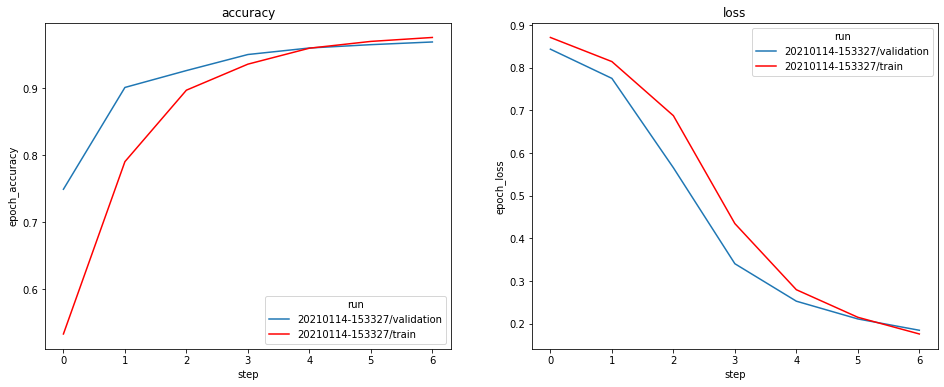
\includegraphics[width=15cm]{kapitel5/acur.png}
    \caption[Vergleich der Genauigkeit mit dem Verlust]{Blau: Validationsdaten. Rot: Trainingsdaten. Links: Die Genauigkeit der Trainings- und Testdatensätze kommt mit jeder Epoche näher und steigt. Rechts: Beide Verlustfunktionen nehmen ab. Während aller Epochen ist eine leichte Überanpassung zu sehen, welches jedoch immer mehr ausgeglicehener wird.}
    \label{Kap5:Val}
\end{figure}


\subsection{Umwandlung und Export in ein Webformat}
%(mit Vocab.json)
\subsection{Schluss}